\documentclass[twocolumn,showpacs,floatfix,longbibliography]{revtex4-1}
\usepackage{graphicx}
\usepackage{bm} % bold math
\usepackage{amssymb} % use this package to enable \nrightarrow command
\usepackage{amsmath} % use this package to enable \xrightarrow command
\usepackage{braket} % use for Dirac bra-kets : \rangle \labgle & \mid
\usepackage{natbib} % bibtex package
\usepackage{hyperref}


\begin{document}

\title{Skyrmion-induced bound state in a superconductor}

\author{Sergey S. Pershoguba$^{1}$}
\author{Sho Nakosai$^{1,2}$}
\author{Alexander V. Balatsky$^{1,3}$}
\affiliation{$^1$Nordita, Center for Quantum Materials, KTH Royal Institute of Technology, and Stockholm University, Roslagstullsbacken 23, S-106 91 Stockholm, Sweden}
\affiliation{$^2$Department of Applied Physics, University of Tokyo, Tokyo 113-8656, Japan}
\affiliation{$^3$Institute for Materials Science, Los Alamos National Laboratory, Los Alamos, New Mexico 87545, USA}

\date{\today}


\begin{abstract}
We consider a superconductor (SC) proximity coupled to a 2D ferromagnet (FM) film with a skyrmion configuration of a FM vector. Using the T-matrix calculations as well as numerical modeling we calculate the spin-polarized local density of states (SP LDOS) in the superconductor in the vicinity of the skyrmion. We find that the skyrmion induces a skyrmion bound state (SBS) in SC similar to the well-known Yu-Shiba-Rusinov (YSR) state. The wavefunction of SBS has a power-law spatial decay. Therefore, in the presence of multiple skyrmions, SC could facilitate an effective long-range interaction when the SBS wavefunctions, induced by different skyrmions, overlap.
\end{abstract}

\pacs{ }   

%%%%%%%%%%%%%%%%%%%%%%%%%%%%%%%%%%%%%%%%%%%%%%%%%%%%%%%%%%%%%%%%%%%%%%%%%%

\maketitle
%%%%%%%%%%%%%%%%%%%%%%%%%%%%%%%%%%%%%%%%%%%%%%%%%%%%%%%%%%%%%%%%%%%%%%%%%%%
\paragraph*{Introduction.---} \label{sec:intro}
%%%%%%%%%%%%%%%%%%%%%%%%%%%%%%%%%%%%%%%%%%%%%%%%%%%%%%%%%%%%%%%%%%%%%%%%%%%

Skyrmions, topological particle-like configurations of a continuous vector field, were originally proposed in the context of high-energy physics.  Nevertheless, it was suggested theoretically \cite{Bogdanov1989,Rossler2006} and recently observed experimentally \cite{Muhlbauer2009,Munzer2010,Yu2011,Heinze2011,Seki2012} that skyrmions exist in chiral ferromagnets in the presence of Dzyaloshinkii-Moriya interaction. Due to non-trivial topological properties, skyrmions manifest anomalous transport response to temperature gradients \cite{Jonietz2010} and electric field \cite{Neubauer2009}. Recently, Hamburg group demonstrated a controllable writing and deleting of single skyrmions on the surface of PdFe bilayer \cite{Romming2013,Bergmann2014,Romming2015}. Coupling of magnetic films with skyrmions to novel materials holds a new promising avenue. For example, interplay of a magnetic skyrmion and a topological insulator was recently considered in Ref.~\cite{Hurst2015}. These developments show that skyrmions hold a great promise in applications such as spintronics, memory devices, etc \cite{Fert2013,Nagaosa2013}. 


In parallel, there has been an immense amount of interest recently in SC-FM heterostructures aimed at engineering topological SC \cite{Alicea2012}. Discovery of the topological SC entails existence of Majorana edge modes, which would pave the way to realizing topological quantum computing \cite{Nayak2008}. So, motivated by the interest in skyrmions, on the one hand, and SC-FM heterostructures, on the other, we connect the two fields in the current work. Few works have considered skyrmions in the context of superconductivity. Reference~\cite{Garaud2011} studied the skyrmion-defects in the multiband superfluids and SCs. Paper \cite{Nakosai2013} discussed a possibility of realizing a topological SC using a skyrmionic lattice. The Josephson current through a magnetic skyrmion structure was considered in Ref.~\cite{Yokoyama2015}. However, none of the papers considered the conceptually simplest case of interaction between a single skyrmion and SC, which is the subject of the discussion below.

%%%%%%%%%%%%%%%%%%%%%%%%%%%%%%%%%%%%%%%%%%%%%%%%%%%%%%%%%%%%%%%%%%%%%%%%%%%
\begin{figure} \centering
(a) 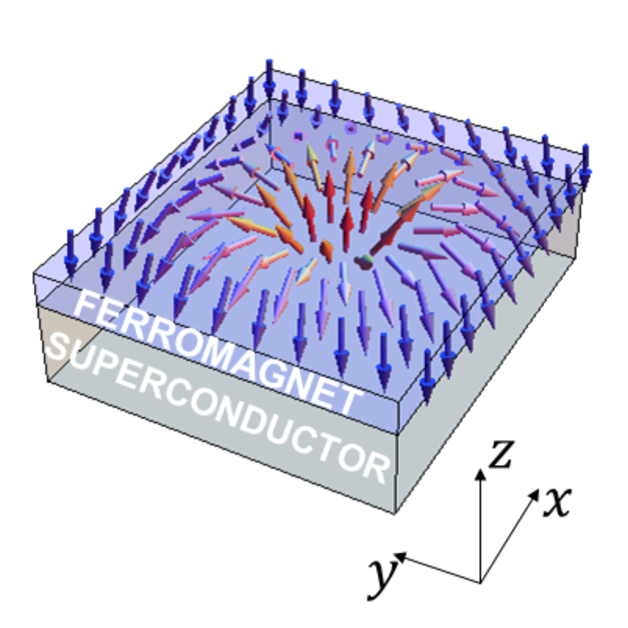
\includegraphics[width=0.4\linewidth]{SkyrmA}  
(b) 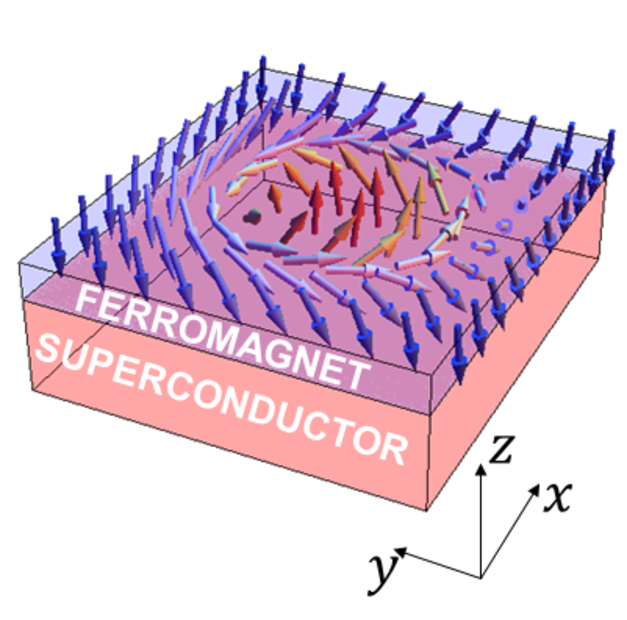
\includegraphics[width=0.4\linewidth]{SkyrmB} \\
(c) 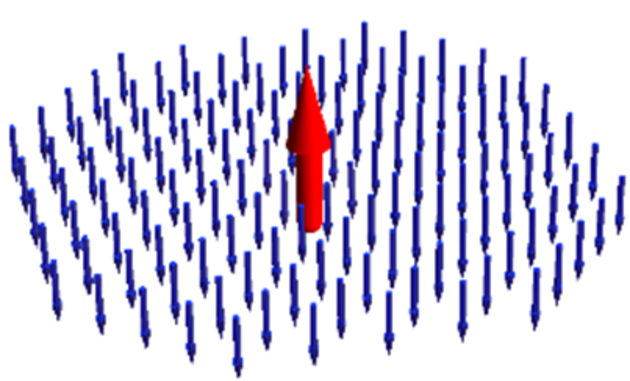
\includegraphics[width=0.4\linewidth]{fig1c}
\caption{(Color online.) (a,b) Ferrormagnetic (FM) film with a skyrmion proximity coupled to a superconductor (SC). (a) N\'eel-type (hedgehog) skyrmion.  (b) Bloch-type (spiral) skyrmion. (c) Sketch of an approximation of a skyrmion as a local magnetic moment floating in a ``ferromagnetic sea''.} \label{fig:skyrmion}
\end{figure}
%%%%%%%%%%%%%%%%%%%%%%%%%%%%%%%%%%%%%%%%%%%%%%%%%%%%%%%%%%%%%%%%%%%%%%%%%%



%%%%%%%%%%%%%%%%%%%%%%%%%%%%%%%%%%%%%%%%%%%%%%%%%%%%%%%%%%%%%%%%%%%%%%%%%%%
\begin{figure} \centering
%	(a)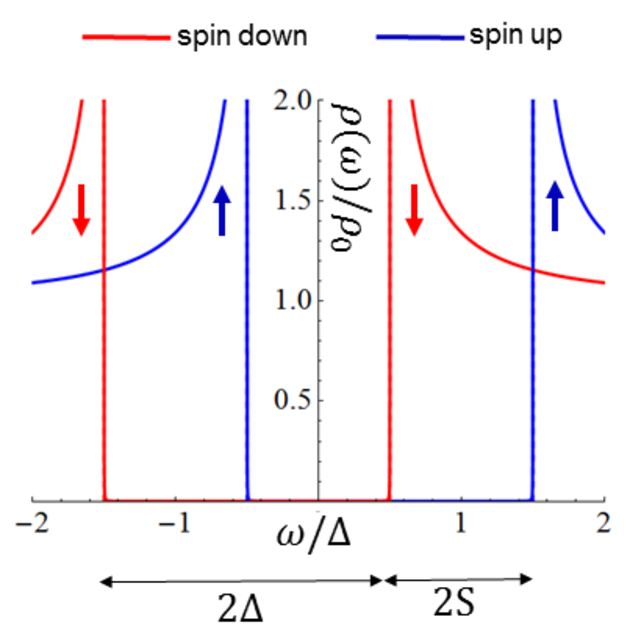
\includegraphics[width=0.25\linewidth]{LDOSa} \hspace{0.1cm}
	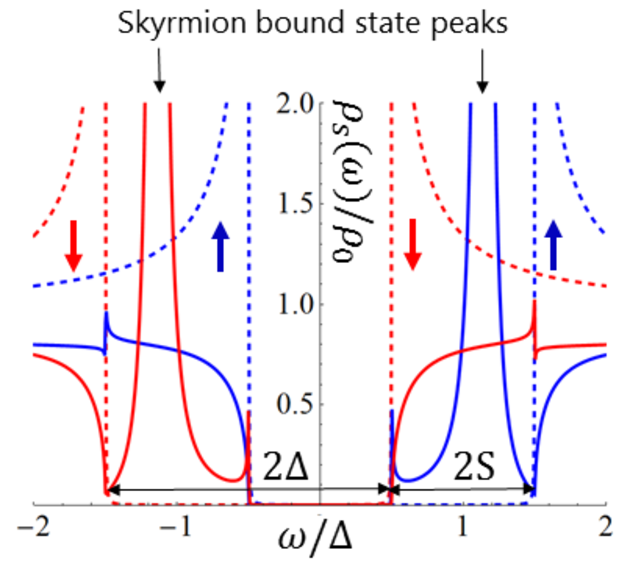
\includegraphics[width=0.7\linewidth]{fig2} 
	\caption{(Color online) Spin-polarized local density of states (SP LDOS) of SC away from the skyrmion (dashed) and at the skyrmion core (solid). The color of the curves encodes the spin polarization: blue for spin up and red for spin down as indicated by the arrows. The figure is obtained by using a model given by Eqs.~(\ref{tm1}) and (\ref{ldos}) for the parameters $2S = \Delta = 0.1 \mu$, $R = 2.5/p_F$, $S_0 = 5SR^2$, and $S_1 = 0.5 SR^3$.} \label{fig:LDOS}
\end{figure}
%%%%%%%%%%%%%%%%%%%%%%%%%%%%%%%%%%%%%%%%%%%%%%%%%%%%%%%%%%%%%%%%%%%%%%%%%%


In the current paper, we consider a FM film with a skyrmion proximity coupled to SC as shown in Fig.~\ref{fig:skyrmion}. We search for the states in SC localized around a skyrmion in a series of approximations. First we consider a limit of a small skyrmion, i.e. $R\ll \xi_{\rm sc}$, in which case we approximate the skyrmion as a point magnetic moment. Using this simplified model, we do an analytical T-matrix calculation and find that skyrmion induces a bound state in the SC in a close analogy with the well-known Yu-Shiba-Rusinov states \cite{Yu,Shiba,Rusinov,Balatsky2006}. We find that SBS induces a resonance with a finite spectral width in a spin-polarized local density of states (SP LDOS). In contrast with the conventional YSR states, which are short-range, the SBS state is a long-range state with a powerlaw decay. Therefore, in the presence of multiple skyrmions, the SC could mediate an effective long-range interaction between skyrmions \cite{Yao2014,Shytov2009} when the SBS states overlap. Later, we relax the requirement $R\ll \xi_{sc}$ and calculate LDOS and the wavefunctions for $R\sim \xi_{sc}$ numerically. We find that the SBS peak is populated by the multiple quasilocalized states corresponding to different angular momenta. 


%%%%%%%%%%%%%%%%%%%%%%%%%%%%%%%%%%%%%%%%%%%%%%%%%%%%%%%%%%%%%%%%%%%%%%%%%%%
\paragraph*{Single skyrmion in a FM film.---} \label{sec:skyrmion}
%%%%%%%%%%%%%%%%%%%%%%%%%%%%%%%%%%%%%%%%%%%%%%%%%%%%%%%%%%%%%%%%%%%%%%%%%%


Consider a FM film with the magnetization described by a three-dimensional vector $\bm S(\bm r) = (S_x,S_y,S_z)$ dependent on a two-dimensional spatial coordinate $\bm r = (x,y)$. The topological configurations of the field $\bm S(\bm r)$ shown in Fig. \ref{fig:skyrmion}(a) and (b) are referred to as skyrmions.  Depending on a specific FM material, two disctinct types of skyrmions are observed in experiment: the N\'eel (hedgehog) skyrmion and Bloch (spiral) skyrmion shown in Fig.~\ref{fig:skyrmion}(a) and (b), respectively. Although, the two types of skyrmions differ significantly in the orientation of the in-plane spins both are characterized by the same topological charge
\begin{align}
	Q = \frac{1}{4\pi} \int d^2r \, \hat {\bm S}\cdot (\nabla_x\hat {\bm S}\times\nabla_y\hat {\bm S})=1,\quad  \hat {\bm S}= \frac{\bm S}{S}. 
	\label{topCharge}
\end{align}
Thus, one can transform a Neel skyrmion into a Bloch skyrmion by a mental $\pi/2$ rotation  \footnote{\label{footnote:Rotation} Note that for the case of a spin-singlet SC given by Eq.~(\ref{ham}), the Bloch and the Neel skyrmions are equivalent since they can be related by a continuous $\pi/2$-rotation around the $z$-axis in the spin space $U = \exp(-i\pi\sigma_z/4)$. In the presence of either the spin-triplet pairing or the spin-orbit interaction, the effects of the two types of skyrmions are different.} of the FM vector around the $\hat {\bm z}$ axis in the spin space without changing a topological charge~(\ref{topCharge}). It would be intriguing to have materials that could exhibit a tunable transition between the two distinct types of skyrmions. 


%%%%%%%%%%%%%%%%%%%%%%%%%%%%%%%%%%%%%%%%%%%%%%%%%%%%%%%%%%%%%%%%%%%%%%%%%%%
\paragraph*{Superconductor proximity coupled to a ferromangetic film.--- }  \label{sec:model}
%%%%%%%%%%%%%%%%%%%%%%%%%%%%%%%%%%%%%%%%%%%%%%%%%%%%%%%%%%%%%%%%%%%%%%%%%%
Let us consider a heterostructure of a SC and FM with a skyrmion as shown in Fig.~\ref{fig:skyrmion}(a) and (b). The SC is described by the 4-by-4 Bogolyubov-de Gennes (BdG) Hamiltonian 
\begin{align}
 H &= \xi(\bm p)\tau_z+\Delta \tau_x - \bm S(\bm r)\cdot\bm\sigma, \label{ham} \\
   & \xi(\bm p) = \frac{\bm p^2}{2m}-\mu,\quad \bm p = -i(\nabla_x,\nabla_y).
\end{align}
Here, $\xi(\bm p)$ describes the kinetic energy and $\Delta$ - the self-consistent supeconducting gap, which we assume uniform in space; the term $\bm S(\bm r)\cdot\bm\sigma$ describes the proximity coupling between the FM film and SC. We assume that the Zeeman splitting $S(\bm r)$ does not exceed the SC gap $\Delta$. The Pauli matrices $\bm \tau$ and $\bm \sigma$ act, respectively, in the particle-hole and spin subspaces of the four-component spinor $\Psi = (\psi_\uparrow,\psi_\downarrow,\psi^\dagger_\downarrow,-\psi^\dagger_\uparrow)^T$. We consider a case with a single N\'eel skyrmion \cite{Note1} centered at $\bm r = 0$, and, so, assume the following profile of the FM vector
\begin{align}
	\bm S(\bm r) &= S\left[ \cos\phi(\bm r) \sin\theta(\bm r),\, \sin\phi(\bm r)\sin\theta(\bm r),\,\cos\theta(\bm r)\right],\nonumber  \\   
	\phi(\bm r) &= \arctan(y/x),\quad \theta(\bm r) = \pi \left[ 1-\exp\left( -\frac{r^2}{R^2} \right) \right], \label{conf}	
\end{align}
where $R$ defines an effective radius of a skyrmion \footnote{We expect that a different spatial dependency of azimuthal angle (\ref{conf}) will not change the results significantly.}. 
%The ferromagnetic vector varies from $\bm S(0) = S\hat{\bm z}$ in the center of the skyrmion to $\bm S(\infty) = -S\hat{\bm z}$ away from the skyrmion.
Let us compare the relevant spatial scales of the problem: the SC coherence length $\xi_{\rm sc} \approx v_F/\Delta$, the skyrmion radius $R$, and the Fermi length $p_F^{-1}$. Both the scales $\xi_{\rm sc}$ and $R$ can vary from tens of nanometers to a micron depending on a specific material, whereas the Fermi length $p_F^{-1}$ is typically smaller than the other two scales. Let us first comment on the regime of the large skyrmion radius, i.e. $R\gg \xi_{\rm sc}$. In this case, the skyrmion can be viewed as a large FM domain pointing in the direction opposite to the rest of the system. Such a regime could be intriguing in the context of topological SC~\cite{Alicea2012}. For instance, it was recently shown \cite{Klinovaja2013} that a helical texture of spins in a one-dimensional (1D) chain of magnetic atoms on a surface of a SC generates an effective Rashba-like spin-orbit interaction responsible for the Majorana edge modes. Similar effective spin-orbit interaction is generated near a skyrmion and could give rise to non-trivial edge states localized at the edge of the skyrmion. We leave the discussion of this intriguing scenario to future works. In the current paper, we focus on the case of relatively small skyrmions, i.e. $R\le \xi_{sc}$. 


%Although the two distincdifferent types of skyrmions are obseved in different materials, nvat We also characterize the skyrmion fields by the zeroth and first moments
%The zeroth moment $\bm S^{(0)} = S_{\rm e} \hat{\bm z}$ characterizes the effective out-of-plane magnetic moment of the skyrmion and is equal for the two skyrmions shown in Fig.~{\ref{fig:skyrmion}}(a) and (b). Whereas, the first-order moment $S^{(1)}_{ij}$ characterizes the in-plane pattern of the ferromagnetic vector $\bm S(\bm r)$. Note that for the cylindrically symmetric field $S(\bm r)$, the first order moment defined in Eq.~(\ref{S1}) can be expanded in the symmetric and antisymmetric parts 
%\begin{equation}
%	S^{(1)}_{ij}=S_{\rm m}\,\delta_{ij} + S_{\rm a}\,\epsilon_{ijz}
%\end{equation}	
%The skyrmions shown in Fig.~\ref{fig:skyrmion}(a) and (b) have monopole $S_{\rm m}$ and anapole $S_{\rm a}$ moments correspondingly, hence the name of the skyrmions. However the two types of the skyrmions have the same topological charge~(\ref{topCharge}) and can be continuosly deformed into each other. 





%%%%%%%%%%%%%%%%%%%%%%%%%%%%%%%%%%%%%%%%%%%%%%%%%%%%%%%%%%%%%%%%%%%%%%%%%%
\begin{figure} \centering
	(a)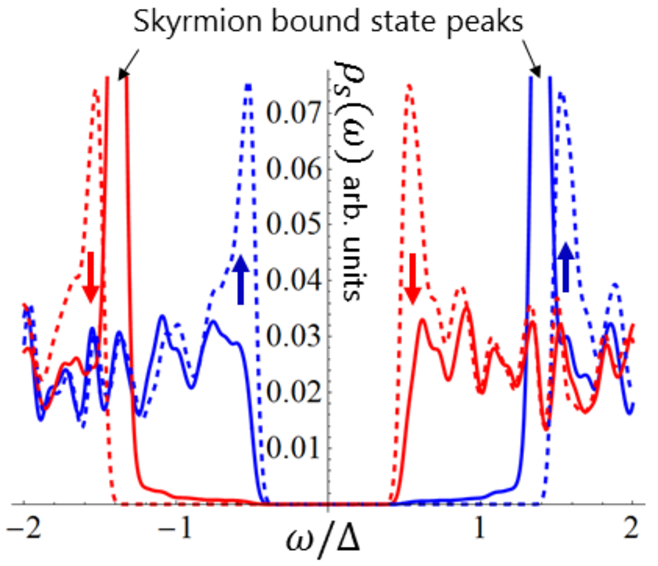
\includegraphics[width=0.7\linewidth]{fig3a} \\  
	(b)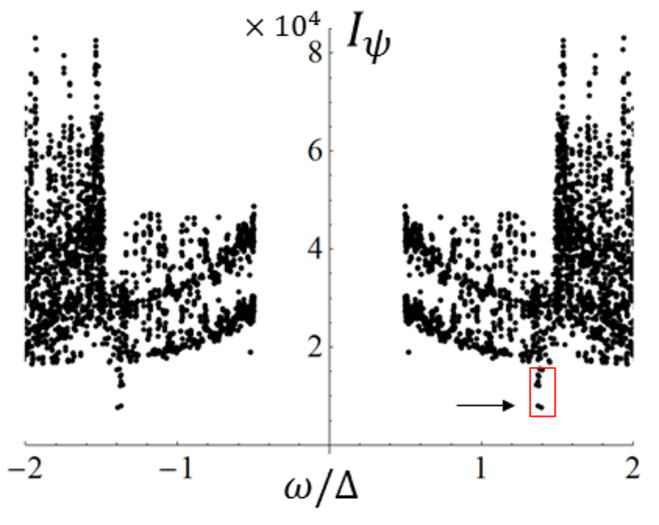
\includegraphics[width=0.7\linewidth]{fig3b} 
	\caption{(Color online) Numerical modeling of a skyrmion. (a) Spin-polarized LDOS at the skyrmion core (solid) and away from the skyrmion (dashed).  (b) Participation ratio representing a measure of localization of  the BdG wavefunctions. The wavefunctions corresponding to the red dots are shown in Fig.~\ref{fig:wavefunction} in the panels indicated by the letters.} \label{fig:LDOSNumerics}
\end{figure}
%%%%%%%%%%%%%%%%%%%%%%%%%%%%%%%%%%%%%%%%%%%%%%%%%%%%%%%%%%%%%%%%%%%%%%%%%%


%%%%%%%%%%%%%%%%%%%%%%%%%%%%%%%%%%%%%%%%%%%%%%%%%%%%%%%%%%%%%%%%%%%%%%%%%%%
\paragraph*{Skyrmion as a local magnetic moment.---} \label{sec:analytics}
%%%%%%%%%%%%%%%%%%%%%%%%%%%%%%%%%%%%%%%%%%%%%%%%%%%%%%%%%%%%%%%%%%%%%%%%%%%
Let us consider a case of a small skyrmion, i.e. $R\ll\xi_{\rm sc}$. In this limit, the SC cannot ``resolve'' the fine details of the field $\bm S(\bm r)$. In the spirit of the multipole expansion used in electrodynamics, we approximate the original skyrmion configuration~(\ref{conf}) as a point magnetic moment floating in a ``ferromagnetic sea'' as illustrated in Fig.~\ref{fig:skyrmion}(c)
\begin{align}
	\bm S_{\rm approx}(\bm r) & =  - S \hat{\bm z} + S_0 \hat{\bm z} \delta^2(\bm r),  \label{vr}
\end{align}
where $S_0$ is the zeroth moment of $\bm S(\bm r)$ \footnote{The elegant multipole expansion captures the salient features of the problem. Because of its simplicity, we use the multipole approximation even beyond its formal domain of validity: $R<p_F^{-1}$ and $R\ll \xi_{sc}$. In the end of the paper, we present an exact numerical modeling and find a close agreement with a multipole analytical treatment.}
\begin{align}
	S_0 = \int  d^2r \, \left[\bm S(\bm r)-\bm S(\infty)\right]_z  \quad \sim \,\,\,SR^2. \label{S0} 
\end{align}

By performing the T-matrix calculation, we solve the model given by Eqs.~(\ref{ham}) and (\ref{vr}), where we treat the local term $S_0 \hat{\bm z} \delta^2(\bm r)$ as a perturbation. We include the constant background magnetization $-S\hat{\bm z}$ in the BdG Hamiltonian $h(\bm p) = \xi(\bm p)\tau_z+\Delta \tau_x +  S\sigma_z$ and calculate an on-site matrix element of the bare Green's function $g(\omega,\bm p) = [\omega-h(\bm p)]^{-1}$ 
 \begin{align}
	 g_{0}(\omega)  =-\pi\rho_0\sum_{\lambda = \pm 1} \frac{1+\lambda\sigma_z}{2}\,\frac{\omega-\lambda S+\Delta\tau_x}{\sqrt{\Delta^2-\left( \omega-\lambda S \right)^2}},  \label{grf}
\end{align}
where $\rho_0 = m/2\pi$ is the density of states. This Green's function describes a SC subject to a uniform background magnetization $-\hat{\bm z} S$ that shifts the spin subbands as shown with the dashed lines in Fig.~\ref{fig:LDOS}.  The density of states contains two interior and two exterior coherence peaks at the energies $\pm(\Delta-S)$ and $\pm(\Delta+S)$ correspondingly.  Using Green's function~(\ref{grf}) we calculate the T-matrix in the presence of a point magnetic moment $V(\bm r)=S_0\,\sigma_z \delta^2(\bm r)$ representing the skyrmion
\begin{align}
	T(\omega) =   \frac{-S_0\sigma_z}{1+S_0\sigma_zg_{0}(\omega)}. \label{tm} 
\end{align}
The poles of T-matrix give the new skyrmion-induced bound states (SBS)
\begin{align}
	E^\pm_{\rm SBS} = \pm\left[S+\Delta \frac{1-\left( \pi\rho S_0 \right)^2}{1+\left( \pi\rho S_0 \right)^2}\right].
	\label{energy}
\end{align}
Let us mention the behavior of the SBS peaks as a function of $S_0$. For small $S_0$, the SBS states split from the outside coherence peaks at the energies $\pm (\Delta+S)$ and move in the direction of the inside coherence peaks with a further increase of $S_0$. Although Eq.~(\ref{energy}) suggests that the SBS states may go inside the actual gap for large enough  $S_0$, i.e. $|E^\pm_{\rm SBS}|<\Delta-S$, the approximation of a skyrmion (\ref{vr}) is no-longer valid in this regime and, thus, does not give a reliable estimate of the SBS energy. In practice, by performing a numerical modeling discussed below, we never observe the SBS peaks inside the actual band gap, i.e. beyond the energies $|E^\pm_{\rm SBS}|>\Delta-S$. The spin-polarization of the SBS states is determined by the spin-polarization of the bulk bands that they split from: the positive (negative) SBS state is ``up'' (``down'') spin-polarized. The found SBS states closely mimic the well-known Yu-Shiba-Rusinov (YSR) states \cite{Yu,Shiba,Rusinov,Balatsky2006} localized around magnetic impurities in SC. The main difference is that the YSR states' energies reside inside the actual spectral gap, whereas the SBS states' energies lie in the window of energies $\Delta+S>|E^\pm_{\rm SBS}|>\Delta-S$. So, the SBS states could hybridize with the bands of the opposite spin polarization.  

Indeed, so far we have considered an approximation of a skyrmion given by Eq.~(\ref{vr}) that includes only $\sigma_z$ matrices. In this approximation, the spin-up and spin-down sectors of the Hamiltonian are decoupled. However let us recall that the original configuration of a FM vector in a skyrmion~(\ref{conf}) has spins in all directions. Specifically, the FM vector $\bm S(\bm r)$ given by Eq.~(\ref{conf}) is purely in-plane for $r = R \sqrt{\ln 2}$. Such in-plane moments generate the terms proportional to $\sigma_x$ and $\sigma_y$ in the Hamiltonian that could couple the spin-up and spin-down sectors of the Hamiltonian. To capture this effect we append the approximation (\ref{vr}) with an additional term 
\begin{align}
	\bm S_{\rm approx}(\bm r) & =  - S \hat{\bm z} + S_0 \hat{\bm z} \delta^2(\bm r)-S_1 \bm \nabla \delta^2(\bm r), \label{vr1}
\end{align}
where  $\bm \nabla = (\nabla_x,\nabla_y)$ and $S_1$ is the first-moment of the original skyrmion configuration\footnote{Note that in the case of the Bloch skyrmion $S_1$ would have a physical meaning of an anapole moment defined as $S_1 = \frac{1}{2}\int  d^2r \, \left\{\left[\bm S(\bm r)-\bm S(\infty)\right] \times \bm r\right\}_z$ }
\begin{align}
	S_1 = \frac{1}{2}\int  d^2r \, \left[\bm S(\bm r)-\bm S(\infty)\right] \cdot \bm r\quad \sim \,\,\,SR^3. \label{S1}
\end{align}
Indeed, the last term in (\ref{vr1}) mimicks the radial in-plane spins of the skyrmion. Similar to calculation above, we solve the Lippmann-Schwinger equation (see details in Supplementary Materials) and calculate the T-matrix 
\begin{align}
	T(\omega) =   \frac{-S_0\sigma_z+S^2_1p_F^2\bar g_{0}(\omega)}{1+S_0\sigma_zg_{0}(\omega)-S^2_1p_F^2\,\bar g_{0}(\omega)\, g_{0}(\omega)}, \label{tm1} 
\end{align}
where for brevity $\bar g_0(\omega) = \frac{1}{2}\sum_{j=x,y} \sigma_j g_0(\omega) \sigma_j $ is the Green's function obtained from Eq.~(\ref{grf}) by substitution $\sigma_z\rightarrow -\sigma_z$, that describes the coupling to bands with opposite spin polarization. Using Eq.~(\ref{tm1}) we calculate SP LDOS 
\begin{align}
	\rho_s & (\omega) = \label{ldos} \\ 
	&-\frac{1}{\pi}\,{\rm Im}{\rm \,Tr} \left\{  \frac{1+\tau_z}{2}\,\frac{1+\sigma_s}{2} \left[g_0(\omega)+g_0(\omega) T(\omega) g_0(\omega)  \right]\right\},\nonumber 
 \end{align}
 where the energy has infinitesimally small imaginary part in the right side of the equation, i.e. $\omega\rightarrow \omega+i\delta$, and $s=x,y,z$ denotes the spin projection axis. We plot LDOS (\ref{ldos}) in Fig.~\ref{fig:LDOS} with solid lines and observe that the peaks corresponding to the SBS resonances have finite spectral width. In order to understand this, we compare Eqs.~(\ref{tm}) and (\ref{tm1}) and observe that the latter contains renormalized numerator and the denominator due to $S_m$. Let us consider poles of the T-matrix~(\ref{tm1}) given by ${\rm det}\left[1+S_{\rm e}\sigma_zg_{0}(\omega)-S^2_{\rm m}p_F^2\,\bar g_{0}(\omega)\, g_{0}(\omega)\right]=0$. The real part of this equation still gives the SBS state given by Eq.~(\ref{energy}). However, since $\bar g_0(\omega)$, which is the Green's function for a flipped spin, is imaginary at the SBS energy, the term $S^2_{\rm m}p_F^2\,\bar g_{0}(\omega)\, g_{0}(\omega)$ becomes imaginary and determines a finite spectral width of SBS resonance. This explains the apparent widening of the spectrum around the SBS state.  Figure~(\ref{fig:LDOS}) allows to compare SP LDOS at the skyrmion core, shown with solid lines, and the energy spectrum far from a skyrmion, shown with dashed lines.   

%%%%%%%%%%%%%%%%%%%%%%%%%%%%%%%%%%%%%%%%%%%%%%%%%%%%%%%%%%%%%%%%%%%%%%%%%%%
\paragraph*{Long-range wave function} \label{sec:wavefuncion} 
%%%%%%%%%%%%%%%%%%%%%%%%%%%%%%%%%%%%%%%%%%%%%%%%%%%%%%%%%%%%%%%%%%%%%%%%%%%

Now let us show that the wave function corresponding to the SBS state has a long-range power-law behavior. Generically, the wave function of an impurity induced state is described by the wave function  
$
	\Psi(\bm r) \sim e^{-ip_Fr+r\sqrt{\Delta^2-\omega^2_\lambda}/v_F}/\sqrt{r},
$
where for brevity $\lambda$ denotes the eigenvalues of $\sigma_z$ operator and $\omega_\lambda = \omega - \lambda S$. The former exponential term describes the fast Friedel oscillations, whereas latter term - behavior at a scale of $\xi_{\rm sc}$. For clarity, let us discuss the positive SBS state, i.e. $\omega = E^{+}_{\rm SBS}$. It lies inside the SC gap for the spin-up subsystem, i.e. $\omega_+<\Delta$, and, so, the latter exponential term describes the exponentially decaying behavior. However, the SBS state also couples to the background spin-down delocalized band, for which it is supragap state, i.e. $\omega_->\Delta$. Therefore, the square root in the becomes imaginary $\sqrt{\Delta^2-\omega^2_-}=-i\sqrt{\omega^2_- - \Delta^2}$, and, so, wavefunction has an oscillating behavior at a scale $\xi_{sc}$. In colloquial terms, the exponentially localized YSR state hybridizes with the delocalized states and produces a long-range SBS state.


%%%%%%%%%%%%%%%%%%%%%%%%%%%%%%%%%%%%%%%%%%%%%%%%%%%%%%%%%%%%%%%%%%%%%%%%%%
\begin{figure} \centering
	(a)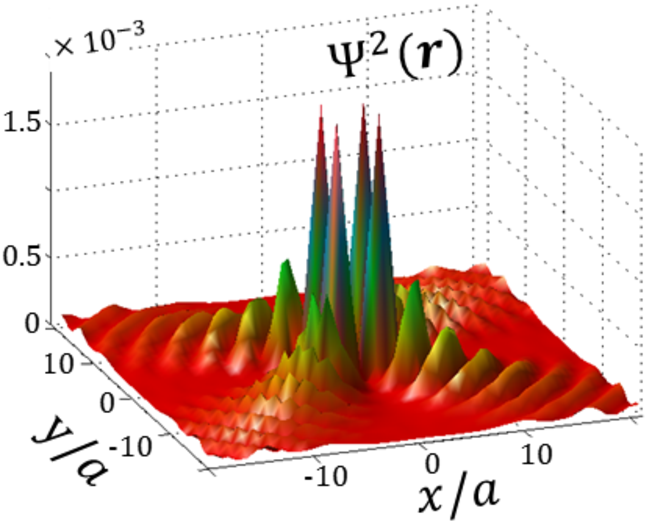
\includegraphics[width=0.43\linewidth]{fig4a}  
	(b)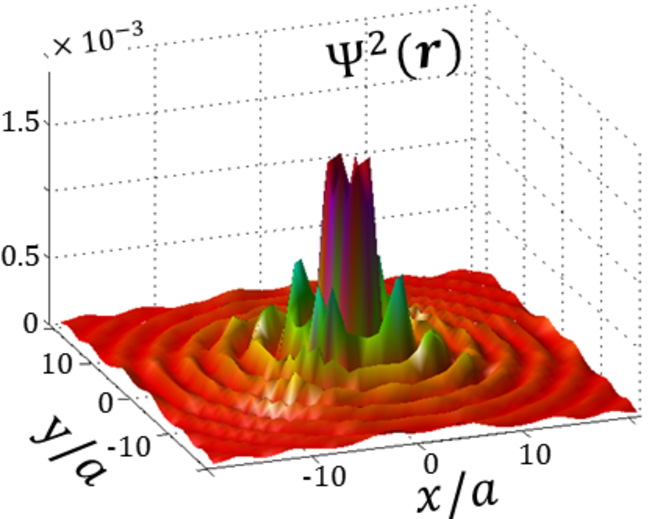
\includegraphics[width=0.43\linewidth]{fig4b} \\
	(c)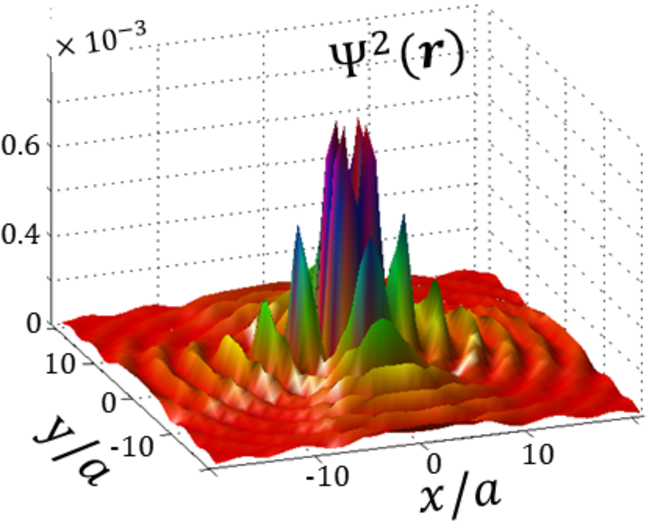
\includegraphics[width=0.43\linewidth]{fig4c}  
	(d)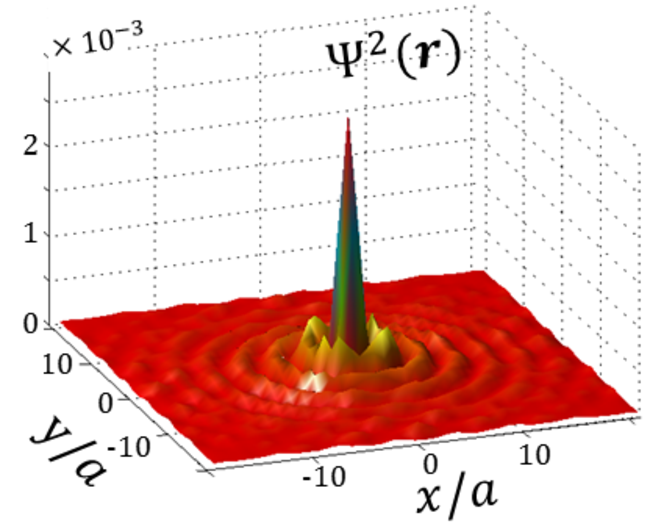
\includegraphics[width=0.43\linewidth]{fig4d} 
	 \caption{(Color online) Spatial profile of the quasilocalized wavefunctions obtained numerically, which are indicated in Fig.~\ref{fig:LDOSNumerics}(b).  } \label{fig:wavefunction}
\end{figure}
%%%%%%%%%%%%%%%%%%%%%%%%%%%%%%%%%%%%%%%%%%%%%%%%%%%%%%%%%%%%%%%%%%%%%%%%%%


%%%%%%%%%%%%%%%%%%%%%%%%%%%%%%%%%%%%%%%%%%%%%%%%%%%%%%%%%%%%%%%%%%%%%%%%%%%
\paragraph*{Numerical analysis.---} \label{sec:numerics} 
%%%%%%%%%%%%%%%%%%%%%%%%%%%%%%%%%%%%%%%%%%%%%%%%%%%%%%%%%%%%%%%%%%%%%%%%%%%
So, approximating a skyrmion as a point impurity, which is valid if $R\ll\xi_{sc}$, we showed that the skyrmion induces resonances in LDOS. We now relax a requirement of small skyrmions and numerically calculate SP LDOS for a large skyrmion $R\sim \xi$. We put the BdG Hamiltonian onto a 2D square lattice with 200-by-200 sites and numerically diagonalize it. The parameters of the tight binding Hamiltonian are $0.1t=\Delta=2S$, $\mu = -3t$, $t$ is a nearest neighbour tunneling amplitude; the radius of skyrmion $R = 6a$, where $a$ is a lattice constant. We numerically calculate SP LDOS and show it in Fig.~\ref{fig:LDOSNumerics}(a). We use the same style as Fig.~\ref{fig:LDOS}: solid (dashed) line represents LDOS on (away from) skyrmion, colors encode opposite spin polarizations. We observe that the calculate LDOS is consistent with the discussion above. Skyrmion does induce a resonance in the LDOS in the energy window in between the original spin-split bands. We also look at the individual normalized BdG eigenstates and calculate the participation ratio
\begin{equation}
	I_\psi =\frac{1}{\sum_{\bm r} |\psi(r)|^4},
	\label{I}
\end{equation}
where the sum is carried over lattice sites $\bm r$. The participation ratio measures a degree of a localization of a wavefunctions: for a localized wavefunction $I_\psi \approx 1$ and for delocalized $I_\psi \approx N$, where $N = 200^2$ is the size of the system. We map $I_\psi$ for all numerical eigenstates and find quasilocalized states for energies corresponding to the SBS peak. We show the electron part  $|\Psi|^2 = |u_{\uparrow}|^2+|u_{\downarrow}|^2$ of the corresponding wavefunction in Fig.~\ref{fig:wavefunction}. We observe that the states with different angular momenta fill up the SBS peak. 




%%%%%%%%%%%%%%%%%%%%%%%%%%%%%%%%%%%%%%%%%%%%%%%%%%%%%%%%%%%%%%%%%%%%%%%%%%%
\paragraph*{Conclusion and Outlook.---} \label{sec:conclusion}
%%%%%%%%%%%%%%%%%%%%%%%%%%%%%%%%%%%%%%%%%%%%%%%%%%%%%%%%%%%%%%%%%%%%%%%%%%%

In this paper, we predict a new skyrmion bound state (SBS) in SC proximity coupled to the FM film with a skyrmion. We calculate SP LDOS and show the signatures of SBS in the tunneling spectrum that coule be measured by the spin-polarized scanning tunneling microscopy (SP STM). The skyrmion typically induces a resonance in between the spin-split coherence peaks corresponding to the opposite spin polarizations. We show that the wavefunction of SBS is quasilocalized, i.e. decays as $1/\sqrt{r}$. Thus in the case of the two skyrmions, their SBS wavefunctions will overlap and induce a long-range interaction between skyrmions \cite{Yao2014,Menard2015}. This will be explored in a following publication. 

We hope that the current paper will be a first step in studying SC-skyrmionic heterostructures and motivate further research. There are intriguing questions in this direction. For instance, SC could in induce effective Dzyaloshinkii-Moriya especially for non-centrosymmetric materials and, thus, stabilize the skyrmionic phase. It would be interesting to explore the connection with the topological SC hybrid systems \cite{Alicea2012}. Superconductivity could potentially endow the skyrmion with a non-trivial statistics by captivating a Majorana fermion \cite{Kim2015}. 

%A number of recent theoretical papers   suggest that superconductivity could provide a strong coubling between the localized magnetic moments. Therefore, superconductivity could potentially be used to stabilize the skyrmionic phase by, e.g., inducing an effective Dzyaloshinskii-Moriya interaction in non-centrosymmetric materials. On of the outcomes of the current paper is that superconductivity could, indeed, mediate a long-range effective interaction between the skyrmions and, thus, affect their dynamics. 


We thank  R.~Wiesendanger, Fujimoto, J.~Zang, A.~Saxena, H. Hurst, and Y. Tserkovnyak for valuable discussions and comments. This work was supported by the US DOE BES E304, ERC DM-321031 and KAW (S.S.P. and A.V.B.). 

\newpage

%%%%%%%%%%%%%%%%%%%%%%%%%%%%%%%%%%%%%%%%%%%%%%%%%%%%%%%%%%%%%%%%%%%%%%%%%%%%%
%\bibliographystyle{apsrev4-1}
\bibliography{Skyrmion}
%%%%%%%%%%%%%%%%%%%%%%%%%%%%%%%%%%%%%%%%%%%%%%%%%%%%%%%%%%%%%%%%%%%%%%%%%%%%%


\appendix 

%%%%%%%%%%%%%%%%%%%%%%%%%%%%%%%%%%%%%%%%%%%%%%%%%%%%%%%%%%%%%%%%%%%%%%%%%%%%%
\section{T-matrix analysis} \label{sec:appendixTMatrix}
%%%%%%%%%%%%%%%%%%%%%%%%%%%%%%%%%%%%%%%%%%%%%%%%%%%%%%%%%%%%%%%%%%%%%%%%%%%%%


In this section, we give an analytic treatment of the skyrmion-induced bound states using the T-matrix approximation. Starting from the Hamiltonian (\ref{ham}) in the second-quantized form, we write the Bogolyubov-de Gennes (BdG) Hamiltonian as 
\begin{align}
	& H_{\rm BdG} = h(\bm p) + V(\bm r),\quad {\rm where}  \label{hbdg} \\
& H(\bm p) = \xi(\bm p)\tau_z+\Delta \tau_x - \bm S(\infty)\cdot\bm\sigma,\quad \bm S(\infty) = -S\,\hat{\bm z}, \nonumber\\
& V(\bm r) = -\left[ \bm S(\bm r)-\bm S(\infty)\right]\cdot\bm\sigma \label{v0}
\end{align}
The momentum-dependent part $H(\bm p)$ describes a superconductor coupled to a spatially uniform FM vector $\bm S(\infty)$, whereas the position-dependent piece $V(\bm r)$ describes the local perturbation due to the skyrmion. Although the specific model is not significant, we assume the following model for the skyrmion centered at the origin $r=0$
\begin{align}
	\bm S(\bm r) &= S\left[ \cos\phi(\bm r) \sin\theta(\bm r),\, \sin\phi(\bm r)\sin\theta(\bm r),\,\cos\theta(\bm r)\right], \nonumber \\   
	\phi(\bm r) &= \arctan(x/y),\quad \theta(\bm r) = \pi \left[ 1-\exp\left( -\frac{r^2}{R^2} \right) \right], 	\label{sr}
\end{align}
where $\phi(\bm r)$ and $\theta(\bm r)$ denote the polar and azimuthal angle of the vector $\bm S(\bm r)$, and $R$ controls the skyrmion size. The superconducting coherence length is usually greater than a typical skyrmion size $R\sim 5$\,nm \cite{Heinze2011,Romming2013,Bergmann2014,Brede2014,Sonntag2014,vonBergmann2015,Romming2015}, i.e. $\xi_{\rm sc}\gg R$. Therefore, the superconductivity does not ``resolve'' the fine details of the skyrmionic configuration of the field  $\bm S(\bm r)$, but rather ``sees'' its long-wavelength characteristics such as the moments described by Eqs.~(\ref{S0}) and (\ref{S1}). Motivated by this logic, we substitute the original skyrmionic field $\bm S(\bm r)$ by its local version 
\begin{equation}
	\bm S(\bm r) - \bm S(\infty) = \left[ S_{\rm e}\, \hat{\bm z} - S_{\rm m}\, \bm \nabla\right] \delta^2(\bm r).
	\label{S}
\end{equation}
Here, in order to relate the moments to the original parameters of the model we subtitute Eq.~(\ref{sr}) in Eqs. (\ref{S0}) and (\ref{S1}) and find 
\begin{align}
	S_{\rm e} &= SR^2 \pi  \left [-\text{Ci}(\pi )+\gamma +\log (\pi )\right] \approx 5.18\, SR^2, \\
	S_{\rm m} &= SR^3 \int_0^{\infty } 2 \pi  t^2 \sin \left(\pi  e^{-t^2}\right) \, dt \approx 6.53\, SR^3.
\end{align}
Equation  (\ref{S}) is convenient for the T-matrix calculation, which we now proceed to. We take into account (\ref{S}) and calculate the Fourier transform of Eq.~(\ref{v0})  
\begin{equation}
	V(\bm p) = -S_{\rm e}\,\sigma_z +  i \,S_{\rm m} \, \bm \sigma\cdot \bm  p,
	\label{vp}
\end{equation}
using which we write an intergal equation for the T-matrix
\begin{align}
	T\left(\bm p^{1},\bm p^{2}\right) &= V \left(\bm p^{1}-\bm p^{2}\right) \nonumber \\
	& +\int \frac{d^2 p'}{\left( 2\pi \right)^2}\, V\left(\bm p^{1}-\bm p'\right) g(\omega,\bm p')  T\left(\bm p',\bm p^{2}\right).
	\label{integEq}
\end{align}
Here, the bare Green's function of the superconductor is defined as 
\begin{align}
	g(\omega,\bm p) = \frac{1}{\omega-h(\bm p)} = \frac{1}{\omega-\xi(\bm p)\tau_z-\Delta \tau_x - S\sigma_z}. \label{g}
\end{align}
Since in the case of the superconductivity we are interested in the scatterings close to the Fermi surface, we use $\bm p^{1} = p_F\, \bm n^{1}$ and $\bm p^{2} = p_F \,\bm n^{2}$, where the in-plane unit vectors $\bm n^{1}$ and $\bm n^{2}$ determine the direction of scattering on the Fermi surface.  Then, we seek the T-matrix in the following form
\begin{align}
	T\left(\bm n^{1},\bm n^{2}\right) &= A + B_i n^{1}_i + C_i n^{2}_j + D_{ij} n^{1}_i n^{2}_j, \label{ansatz}
\end{align}
where  $A,B_i,C_i$ and $D_{ij}$ are the matrices in the four-components space $\sigma\otimes\tau$. We substitute ansatz~(\ref{ansatz}) in the integral Eq.~(\ref{integEq}) and find the T-matrix
\begin{widetext}
\begin{equation}
	T\left(\bm n^{1},\bm n^{2}\right) = \frac{-S_{\rm e}\sigma_z+S^2_{\rm m}p_F^2\bar g_{0}(\omega)+i\,S_{\rm m}\,p_F \,  \bm \sigma\cdot(\bm n^{2}- \bm n^{1}) +S^2_{\rm m}\, p^2_F \, \bar g_{0}(\omega)\,\left(\bm \sigma\cdot\bm n^{2}\right)\,\left(\bm \sigma\cdot \bm n^{1}\right)}{1+S_{\rm e}\sigma_zg_{00}-S^2_{\rm m}p_F^2\,\bar g_{0}(\omega)\, g_{0}(\omega)}, \label{TM}
\end{equation}
\end{widetext}
where the Green's function on-site matrix element in the real space is denoted as 
\begin{align}
	g_{0}(\omega) &   =\int \frac{d^2 p}{\left( 2\pi \right)^2}\, g(\omega,\bm p)  	\label{g0} \\
	 & =-\pi\rho\sum_{\lambda = \pm 1} \frac{1+\lambda\sigma_z}{2}\,\frac{\omega-\lambda S+\Delta\tau_x}{\sqrt{\Delta^2-\left( \omega-\lambda S \right)^2}}, \nonumber \\
	 \bar g_{0}(\omega) & = \frac{1}{2} \sum_{j=x,y}\sigma_j\, g_{0}(\omega)\, \sigma_j.\label{bg0}
\end{align}
For brevity, $\bar g_{0}$ denotes the Green's function obtained from $g_{00}$ by replacing $\sigma_z \rightarrow - \sigma_z$ according to Eq.~(\ref{bg0}). The density of states per spin is denoted as $\rho = m/2\pi$. So, in the presence of the skyrmion, the Green's function becomes
\begin{align}
	G(\omega,\bm p^1,\bm p^2) =& g(\omega,\bm p^1)\,(2\pi)^2\delta(\bm p^1-\bm p^2) \nonumber \\ 
	          &  +g(\omega,\bm p^1) T(\bm p^1,\bm p^2) g(\omega,\bm p^2),
	\label{G}
\end{align}
using which the spin-polarized local density of states (LDOS) can be expressed
\begin{align}
	\rho_s(\omega,\bm r) = -&\frac{1}{\pi}\,{\rm Im}\lim_{\omega\rightarrow \omega+i\delta}{\rm\,Tr} \left[ \frac{1+\tau_z}{2}\,\frac{1+\sigma_s}{2} \right. \label{rhor} \\
	&\left.\int \frac{d^2p^1\,d^2p^2}{\left( 2\pi \right)^4} e^{i\left( \bm p^1-\bm p^2 \right)\bm r} G(\omega,\bm p^1,\bm p^2)\right]\, \nonumber 
\end{align}
where $s=x,y,z$ denotes the spin quantization axis. It can be easily evaluated for instance at the skyrmion core, i.e. at $\bm r=0$,
\begin{align}
	& \rho_s(\omega,0) = -\frac{1}{\pi}\,{\rm Im}\lim_{\omega\rightarrow \omega+i\delta}{\rm \,Tr} \left\{  \frac{1+\tau_z}{2}\,\frac{1+\sigma_s}{2}  \right. \label{spldos} \\
	&\left.\left[g_0(\omega)+g_0(\omega)  \frac{-S_{\rm e}\sigma_z+S^2_{\rm m}p_F^2\bar g_{0}(\omega)}{1+S_{\rm e}\sigma_zg_{00}-S^2_{\rm m}p_F^2\,\bar g_{0}(\omega)\, g_{0}(\omega)} g_0(\omega)  \right]\right\}\, \nonumber 
\end{align}

%%%%%%%%%%%%%%%%%%%%%%%%%%%%%%%%%%%%%%%%%%%%%%%%%%%%%%%%%%%%%%%%%%%%%%%%%%%
%\begin{figure*} \centering
%	(a)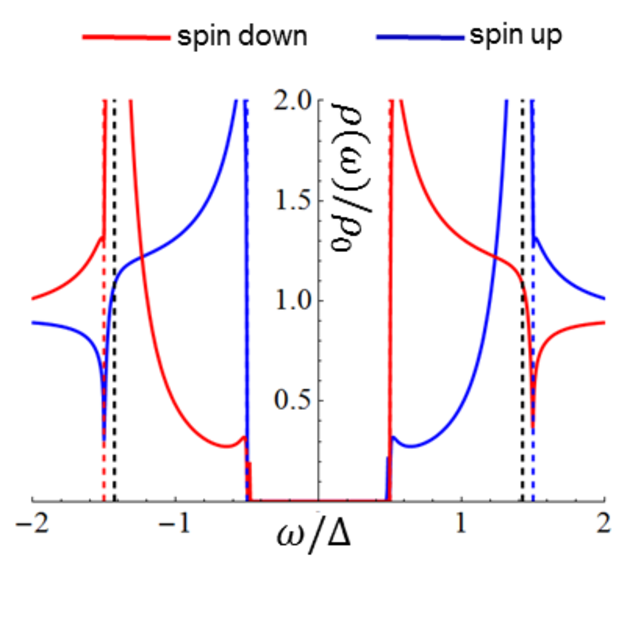
\includegraphics[width=0.25\linewidth]{ApLDOSa} \hspace{0.1cm}
%	(b)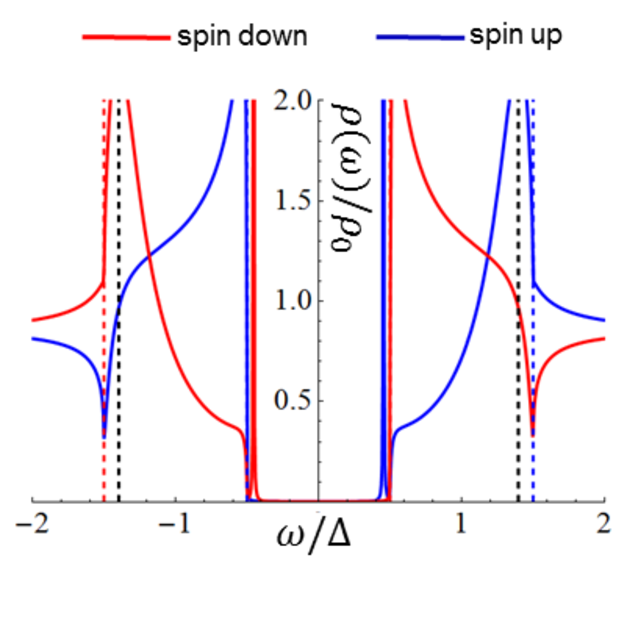
\includegraphics[width=0.25\linewidth]{ApLDOSb} \hspace{0.1cm}
%	(c)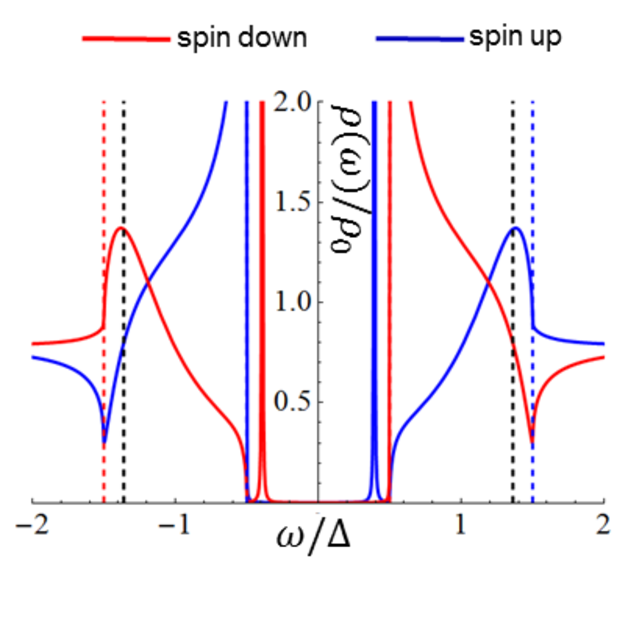
\includegraphics[width=0.25\linewidth]{ApLDOSc} 
%	\caption{(Color online) Spin-polarized local density of states (SP-LDOS)  at the core of the skyrmion. The consequent panels correspond to increasing skyrmion size (a) $R = 1.1 p_F^{-1}$, (b) $R = 1.2 p_F^{-1}$, (c) $R = 1.3 p_F^{-1}$. Other parameters are the same as in Fig.~\ref{fig:LDOS}. } \label{fig:ApLDOS}
%\end{figure*}
%%%%%%%%%%%%%%%%%%%%%%%%%%%%%%%%%%%%%%%%%%%%%%%%%%%%%%%%%%%%%%%%%%%%%%%%%%

%%%%%%%%%%%%%%%%%%%%%%%%%%%%%%%%%%%%%%%%%%%%%%%%%%%%%%%%%%%%%%%%%%%%%%%%%%%%%
%\section{Wave function of the resonance} \label{sec:wf}
%%%%%%%%%%%%%%%%%%%%%%%%%%%%%%%%%%%%%%%%%%%%%%%%%%%%%%%%%%%%%%%%%%%%%%%%%%%%%
%In this section, we discuss the wavefunction corresponding to SBS resonance. The treatment is analogous to the discussion of T-matrix in the previous setion. We write Eq.~(\ref{hbdg}) in the form of the BdG equation in the momentum space
%\begin{align}
%	\left[ \omega - h(\bm p) \right] \Psi(\bm p)= \int \frac{d^2 p'}{\left( 2\pi \right)^2}\,V(\bm p-\bm p')\,\Psi(\bm p'),	\label{bdge}
%\end{align}
%where $\Psi(\bm p)$ is the four-component wave function in the $\sigma\otimes\tau$ space. We substitute Eq.~(\ref{vp}) in the right hand side of Eq.(\ref{bdge}), use the definition of Green's function~(\ref{g}) and obtain 
%\begin{align}
%	\Psi (\bm p) = - g(\bm p) \left( S_{\rm e}\sigma_z +  i S_{\rm m}  \bm \sigma\cdot \bm  p \right)\,\Phi_1 -i\,g(\bm p)S_m\sum\limits_{j=x,y}\sigma_j \Phi_{2j},
%	\label{pwf}
%\end{align}
%where $\Phi_1$ and $\Phi_{2j}$ are the unknown four-component spinors defined self-consistently via wave function as 
%\begin{align}
%	\Phi_1 =  \int \frac{d^2 p'}{\left( 2\pi \right)^2}\, \Psi(\bm p'),\quad \Phi_{2j} =  \int \frac{d^2 p'}{\left( 2\pi \right)^2}\, p'_j\Psi(\bm p').
%	\label{f12}
%\end{align}
%Therefore, we close the equations by substituting~(\ref{pwf}) in Eq.~(\ref{f12}), take the integrals and obtain the following equations for the spinors
%\begin{align}
%	\Phi_1 &= -S_{\rm e} g_0 \sigma_z\Phi_1 - i S_{\rm m} g_{0} \sum_{j=x,y}\sigma_{j} \Phi_{2j}, \label{e1} \\
%	\Phi_{2j} &= \frac{i}{2}S_{\rm m}p_{F}^2 g_0 \sigma_j \Phi_1. \label{e2}
%\end{align}
%We substitute Eq.~(\ref{e2}) in Eq.~(\ref{e1}) and obtain the equation for $\Phi_1$
%\begin{align}
%	\left[1+S_{\rm e} g_0 \sigma_z\,\Phi_1 -  S^2_{\rm m} p_F^2\,g_{0} \bar g_{0} \right] \Psi_1 = 0. \label{le} 
%\end{align}
%This derivation is equivalent to the T-matrix treatment, and, therefore, notice that Eq.~(\ref{le}) corresponds to finding kernel of the denominator of T-matrix~(\ref{TM}). Since the matrix expression in the square brackets contains only $\sigma_z$ and $\tau_x$ matrices, the spinor $\Psi_1$  is an eigenstate of these matrices defined as ${\tau_x \mid \pm\rangle = \pm \mid \pm\rangle}$ and ${\sigma_z \mid \uparrow\downarrow\rangle = \pm \mid\uparrow\downarrow\rangle}$. That is the spinor for the positive SBS state is ${\Phi_{1} = \mid \uparrow\rangle\otimes \mid + \rangle}$ and negative - ${\Phi_{1} = \mid \downarrow\rangle\otimes \mid - \rangle}$, just as for the usual YSR state. We also substiute Eq.~(\ref{e2}) in Eq.~(\ref{pwf}) and obtain
%\begin{align}
%	\Psi(\bm p) &= - g(\bm p) \left( S_{\rm e}\sigma_z +  i S_{\rm m}  \bm \sigma\cdot \bm  p -S^2_{\rm m}p_F^2\bar g_0\right)\Phi_1,  \nonumber \\
%	&= - g(\bm p) \left( S_{\rm e}\sigma_z  - S^2_{\rm m}p_F^2\bar g_0\right)\Phi_1 -   i  S_{\rm m} g(\bm p)\,  \bm \sigma\cdot \bm  p \,\Phi_1. \label{pwf1} 	
%\end{align}
%In order to find the wave function in the real space one has to Fourier transform Eq.~(\ref{pwf1}). It can be done carefully but the resulting equations are bulky and obscure, so we are just going to show that the first term in the second line of Eq.~(\ref{pwf1}) gives exponentially localized wavefucntion, whereas the last term has a powerlaw decay and is thus long-ranged. The key element is finding the Fourier transform of the Green's function which we expand using the projector operators $(1\pm \sigma_z)/2$
%\begin{align}
%	g_{\bm r} &= \int \frac{d^2 p}{\left( 2\pi \right)^2} g(\bm p) =   \sum_{\lambda = \pm} \frac{1+\lambda\sigma_z}{2}\,g_{\bm r}^\lambda \nonumber,\quad{\rm where} \\
%	 g_{\bm r}^\lambda &=\int \frac{d^2 p}{\left( 2\pi \right)^2} \frac{e^{i\bm p \bm r}}{\omega_\lambda -\xi\tau_z-\Delta\tau_x},\,\,\omega_\lambda = \omega - \lambda S.  \label{lle}
%\end{align}
% The integral in Eq.~(\ref{lle}) can be evaluated for $r\gg v_F/\omega_D$ \cite{Pientka2013}, where $\omega_D$ is the Debye energy,
%\begin{align}
%	g^\lambda_{\bm r} = & -\pi\rho\left\{\frac{(\omega_\lambda+\Delta\tau_x)}{2\sqrt{\Delta^2-\omega_\lambda^2}}\left[ f_1(\bm r)+f_2(\bm r) \right] + \tau_x \left[ f_1(\bm r)-f_2(\bm r) \right]\right\}, \nonumber \\
%	& {\rm where}\,\,\, f_1(\bm r) = J_0\left[\left( p_F+ip_\lambda \right)r\right] + H_0\left[\left( p_F+ip_\lambda \right)r\right], \nonumber\\ 
%	& \qquad\quad f_2(\bm r) = J_0\left[\left( p_F-ip_\lambda \right)r\right] - H_0\left[\left( p_F-ip_\lambda \right)r\right], \nonumber\\
%	& \qquad\quad p_\lambda = \frac{\sqrt{\Delta^2-\omega^2_\lambda}}{v_F},
%\end{align}
%where $J_0$ and $H_0$ are the Bessel and Struve functions, $p_F$ - Fermi momentum, $p_\lambda$ characteristic momentum of a superconductor. Although the Green's function in the real space is quite bulky, it has a simple assymptotic behavior at $r\gg \xi_{sc}$
%\begin{equation}
%	g^{\lambda}_{\bm r} \sim \frac{e^{i p_F r}e^{-p_\lambda r}}{\sqrt r}. \label{asym}
%\end{equation}
%The first term describes fast Friedel oscillations, whereas second term - behavior at a scale of the superconducting coherence length $\xi_{sc}$. For the state inside the superconducting gap, i.e. for $|\omega_\lambda|<\Delta$, the latter term the exponential decay. In contrast for the state inside the continuum, i.e. for $|\omega_\lambda|>\Delta$, $p_\lambda$ becomes imaginary, i.e. $p_\lambda = -i\sqrt{\omega^2_\lambda-\Delta^2}/v_F$, and therefore the last exponential term in Eq.~(\ref{asym}) describes periodic oscillations with a period $\Delta r \sim 1/\xi_{sc}$. 

%The polarized SBS state discussed above lies inside the continuum of states corresponding to the opposite spin polarization. Moreover, the last term in Eq.~(\ref{pwf1}) describes the coupling of the state to the continuum of the background delocalized states. Thus, the SBS is expected to have an oscillating power-law rather than decaying behavior as also supported by the numerics. 

\end{document}
